\documentclass[a4paper,14pt]{article}

\usepackage{listings}
\usepackage{xcolor}
\usepackage{graphicx}
\usepackage{cmap}	
\usepackage{tabto}			
\usepackage[T2A]{fontenc}			
\usepackage[utf8]{inputenc}			
\usepackage[english,russian]{babel}	

\title{Lex-BFS}
\date{21.05.2019}
\author{}
\begin{document} 

\maketitle
\section{Введение}
\begin{itemize}
	\item \textbf{BFS} - алгоритм, позволяющий найти кратчайшие пути из одной вершины невзвешенного (ориентированного или неориентированного) графа до всех остальных вершин. В результате работы алгоритма подмножества вершин упорядочиваются по удаленности от исходной, в каждом из подмножеств вершины неупорядочены. 
	\item \textbf{Lex-BFS} - алгоритм,позволяющий дополнительно упорядочить подмножества вершин, полученных в результате работы обычного BFS.
\end{itemize}
\section{Алгоритм Lex-BFS}
	Предполагается, что читатель уже знаком с работой BFS, поэтому описание данного алгоритма опустим.
	\newline
	\newline Как и в обычном BFS, в начале работы алгоритма необходимо указать "стартовую" вершину, из которой мы и запустим обход.
	\newline Заведем очередь, в которой будем хранить некоторые непересекающиеся подмножества(которые мы определим позже) вершин графа.
	\newline В начале работы алгоритма в очереди содержится только множество всех вершин графа. После удаления некоторой вершины $v$ из первого множества в очереди, множество, содержавшее $v$, если оно стало пустым, удаляется из очереди, $v$ добавляется в вывод, а затем каждое множество $M_k$ в очереди заменяется на два: соседи данной вершины - $N_k$ и все остальные вершины. Для этого всех соседей $v$ перемещаем из $M_k$ в $N_k$. $N_k$ помещаем в очереди перед $M_k$. Если $M_k$ пусто, удаляем его из очереди. Затем в качестве $v$ выбирается вершина из первого множества в очереди(в случае, когда в множестве лежит несколько вершин, выбор не имеет значения).
	\newpage Собственно псевдокод(автор не претендует на эффективность, псевдокод предназначен для лучшего понимания алгоритма):
	\newline
	\newline \tab \tab S = queue()
	\newline \tab \tab S.push(V)  //V - множество всех вершин графа
	\newline \tab \tab v = input\underline{ }vertex  //инициализируем стартовую вершину 
	\newline \tab \tab Neighbour //список соседей для каждой вершины
	\newline \tab \tab Output = queue()
	\newline \tab \tab for i in V: //для каждой вершины отмечаем, в каком множестве она лежит
	\newline \tab \tab \quad i.h\underline{ }set = V 
	\newline \tab \tab While not S.empty():
	\newline \tab \tab \quad v.visited = True
	\newline \tab \tab \quad Output.push(v)
	\newline \tab \tab \quad S.front().remove(v)
	\newline \tab \tab \quad if S.front().empty():
	\newline \tab \tab \quad \quad S.pop()
	\newline \tab \tab \quad for i in Neighbour[v]:
	\newline \tab \tab \quad \quad if not i.visited():
	\newline \tab \tab \quad \quad \quad M = i.h\underline{ }set
	\newline \tab \tab \quad \quad \quad if M.divided(): //если множество уже учавстовало в делении на данной итерации- помещаем соседа в предыдущее множество, иначе- создаем новое и помещаем его перед данным
	\newline \tab \tab \quad \quad \quad \quad N = S.predecessor(M)
	\newline \tab \tab \quad \quad \quad else:
	\newline \tab \tab \quad \quad \quad \quad N = set()
	\newline \tab \tab \quad \quad \quad \quad S.place\underline{ }before(M, N) 
	\newline \tab \tab \quad \quad \quad i.h\underline{ }set = N
	\newline \tab \tab \quad \quad \quad M.remove(i)
	\newline \tab \tab \quad \quad \quad N.add(i)	
	\newline \tab \tab \quad \quad \quad if M.empty():
	\newline \tab \tab \quad \quad \quad \quad S.delete(M)
	\newline \tab \tab \quad  v = S.front()[0]
	\newline \tab \tab return(Output)
\section{Разбор полётов}
	 Рассмотрим работу алгоритма на примере, для удобства будем присваивать вершинам лексикографические метки(для соседей начальной вершины это количество вершин($n$) в графе, для всех остальных - текущая метка * 10 + текущее количество необработанных вершин):
	\newpage Пусть дан следующий граф:
	\begin{figure}[h!]
		\centering
		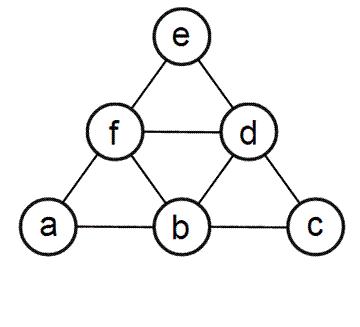
\includegraphics[width=40mm]{img/1.png}
	\end{figure}
	\newline Обрабатываем стартовую вершину и ставим метки:
	\begin{figure}[h!]
		\centering
		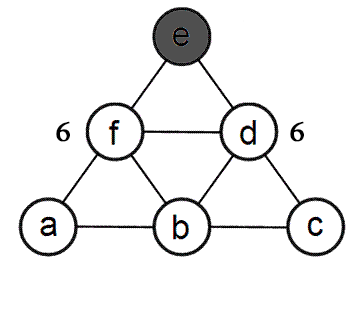
\includegraphics[width=40mm]{img/2.png}
	\end{figure}
	\newline Из двух вершин с одинаковыми метками выберем вершину f:
	\begin{figure}[h!]
		\centering
		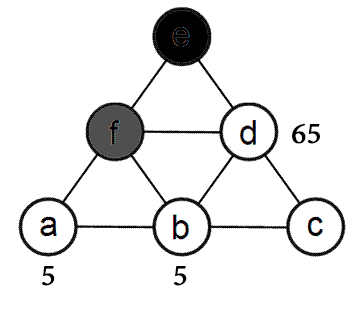
\includegraphics[width=40mm]{img/3.png}
	\end{figure}
	\newline Дальше работа алгоритма ясна:
	\begin{figure}[h!]
		\centering
		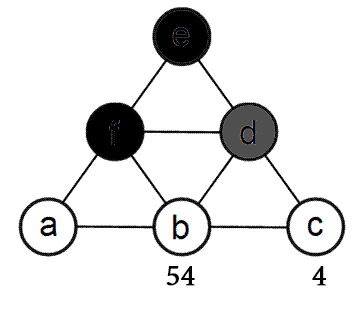
\includegraphics[width=40mm]{img/4.png}
	\end{figure}
	\newpage Ещё одна итерация:
	\begin{figure}[h!]
		\centering
		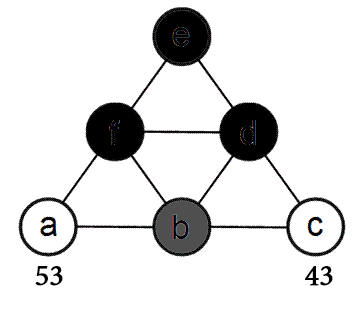
\includegraphics[width=40mm]{img/5.png}
	\end{figure}
	\newline И ещё одна:
	\begin{figure}[h!]
		\centering
		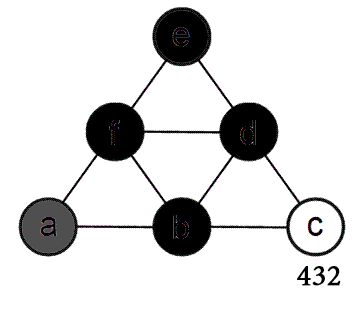
\includegraphics[width=40mm]{img/6.png}
	\end{figure}
	\newline И ещё:
	\begin{figure}[h!]
		\centering
		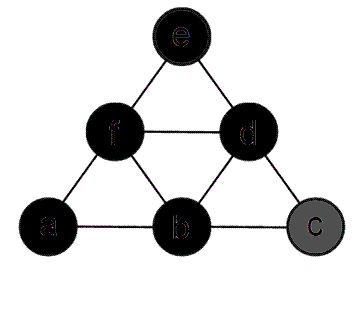
\includegraphics[width=40mm]{img/7.png}
	\end{figure}
	\newline И наконец:
	\begin{figure}[h!]
		\centering
		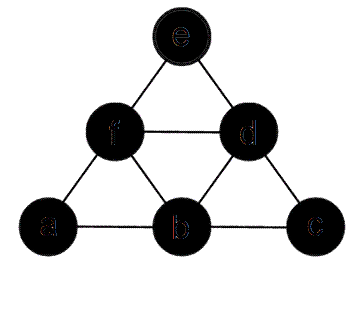
\includegraphics[width=50mm]{img/8.png}
	\end{figure}
	\newline Таким образом на выходе получаем: e, f, d, b, a, c.
	\newline Отметим также, что если на втором шаге выбрать вершину d, то вывод изменится: e, d, f, b, c, a.
\section{Оценка сложности}
	 Интуитивно понятно, что алгоритм не сильно отличается от стандартного поиска в ширину, и его вычислительная сложность также является линейной.
	\newline
	\newline Проведём, однако, оценку:
	\newline
	\newline Каждая вершина графа обрабатывается ровно один раз, аналогично каждое ребро обрабатывается единственный раз при обходе соседей некоторой вершины, в предположении, что добавление и удаление элементов множества, а также добавление элемента в очередь происходит за $O(1)$, получаем искомую сложность в $O(|V|+|E|)$.
\section{Приложения к lex-BFS: тестирование графа на хордальность}
	\textbf{Некоторые базовые понятия и определения:} 
\begin{itemize}
	\item \textbf{Хордальный граф} - граф, каждый из циклов длины больше 3 которого, имеет хорду (ребро, соединяющее две вершины цикла, но не являющееся его частью).
	\begin{figure}[h!]
		\centering
		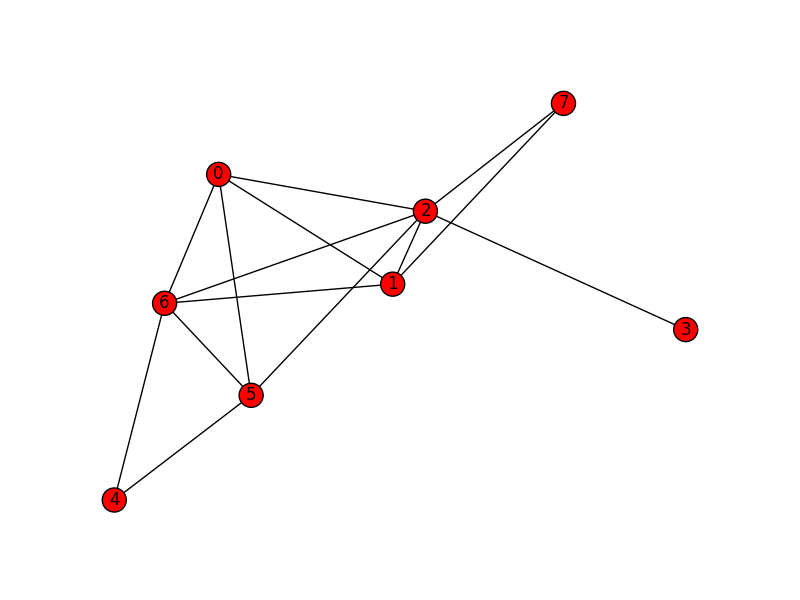
\includegraphics[width=40mm]{img/hord.png}
	\end{figure}
	\item \textbf{Клика} - подмножество вершин неориентированного графа, любые две из которых соединены ребром.
	\begin{figure}[h!]
		\centering
		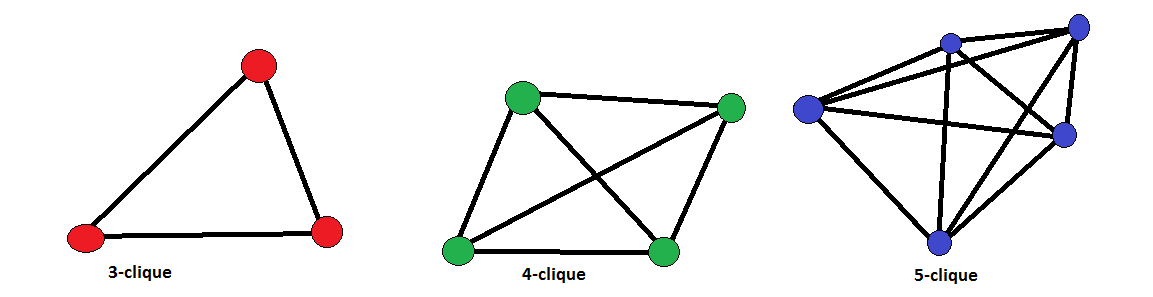
\includegraphics[width=60mm]{img/clique.png}
	\end{figure}
	\item \textbf{Совершенный порядок исключения} - порядок вершин графа, такой, что для каждой вершины $v$, $v$ и соседи $v$, находящиеся после $v$ в упорядочении, образуют клику. Граф хордален тогда и только тогда, когда имеет совершенный порядок исключения.
\end{itemize}
	 \textbf{Алгоритм теста на хордальность:}
	\newline
	\newline  \tab \tab  Пусть $p$ - последовательность вершин, полученная в результате lex-BFS, $RN(v)$ - соседи $v$ в исходном графе, лежащие правее $v$ в $p$, $P(v)$ - родитель, самая левая вершина из $RN(v)$ в $p$. 
	\newline  \tab \tab  Пусть $T$ - дерево, составленное из родительских вершин. Обойдём $T$ обратным обходом. Для каждой вершины $v$ в обходе будем проверять, выполнено ли условие: $(RN(v)\setminus P(v)) \subseteq RN(P(v))$
	\newline  \tab \tab Если условие выполнено для каждой вершины T, то $p$ - совершенный порядок исключения, а граф является хордальным. Если условие не выполнилось хотя бы для одной вершины, то граф хордальным не является.
	\newline
	\newline  \textbf{Доказательство корректности:}
	\newline
	\newline  \tab \tab $\Rightarrow$ Пусть граф не является хордальным, покажем, что найдется вершина, для которой условие не будет выполняться. Так как граф не является хордальным, найдётся вершина $v$, для которой $\{v\} \cup RN(v)$ не является кликой. Без ограничения общности, выберем самую правую вершину в $p$ с таким свойством. По выбору $v$ мы получаем, что во множестве соседей родителя $v$ не содержится некоторая вершина, являющаяся соседом $v$, следовательно условие не выполняется.
	\newline  \tab \tab $\Leftarrow$ Пусть $p$ - совершенный порядок исключения, тогда  $\{v\} \cup RN(v)$ - клика, где $v$ - самая левая её вершина в $p$, а родитель $v$ - самая левая, идущая за $v$, её вершина в $p$, а значит условие выполняется.
	\newline 
	\newline  \textbf{Оценка сложности:}
	\newline
	\newline  Докажем оценку сложности в $O(|V| + |E|)$:
	\newline
	\newline $p$ вычисляется за $O(|V| + |E|)$ в силу оценки на lex-BFS, остаётся оценить сложность вычисления $RN(v)$ и $P(v)$. Инициализируем $RN(v)$ пустым списком, а $P(v)$ специальным значением, означающим отсутсвие предка. Для каждой вершины пройдемся по соседям, добавим в $RN(v)$ соседа, если он лежит правее $v$, самого левого из таких соседей добавим в $P(v)$. Заметим, что $RN(v)$ - антисимметричное отношение, а значит, если мы не добавляем некоторого соседа $u$ вершины $v$ в $RN(v)$, то будем добавлять $v$ в $RN(u)$, при любом добавлении $u$ в $RN(v)$ или наоборот будем проверять: не лежит ли добавленная вершина левее родителя, и при необходимости будем обновлять родителя. Таким образом, каждую вершину и каждое ребро мы обработаем ровно один раз. Считая, что операции со множествами работают за $O(1)$, получаем необходимую оценку.   
\end{document} 



